\documentclass[12pt]{beamer}

\usepackage[T1]{fontenc} 
\usepackage[utf8]{inputenc}
\usepackage[frenchb]{babel}
\usepackage{amsmath}
\usepackage{xcolor}
\usepackage{listings}
\usepackage{graphicx}
\usepackage{animate}
\usepackage{wrapfig}
\usepackage{movie15}
% * * * * * * * * * * * * * * CHOIX DU THEME  * * * * * * * * * * * * * * * * *
\usepackage{beamerthemeMadrid}       

% * * * * * * * * * * * * * LA BARRE DE NAVIGATION  * * * * * * * * * * * * * *
\setbeamertemplate{navigation symbols}{%
	\insertslidenavigationsymbol%
	\insertframenavigationsymbol%
	\insertsubsectionnavigationsymbol%
	\insertsectionnavigationsymbol%
	\insertdocnavigationsymbol%
	\insertbackfindforwardnavigationsymbol%
}

% * * * * * * * * * * * * * * * * * TEXTPOS * * * * * * * * * * * * * * * * * *
\usepackage[absolute,showboxes,overlay]{textpos}
\TPshowboxestrue                                              % affiche le contour des textblocks
\TPshowboxesfalse                                             % fait disparaitre le contour des textblocks
\textblockorigin{2mm}{8mm}                                    % origine des positions pour placer les textblocks

% * * * * * * * * * * * * * * * * * PICTURE * * * * * * * * * * * * * * * * * *
\usepackage{picture}
\setlength{\unitlength}{1mm}  

% * * * * * * * * * * * * * DETAILS DE STYLE  * * * * * * * * * * * * * * * * *
\beamertemplatetransparentcovered      
\setbeamertemplate{itemize item}[ball] 
\setbeamertemplate{itemize subitem}[triangle] 

\logo{
\includegraphics[height=7mm]{images/ustl1.jpg}}     
\renewcommand{\arraystretch}{1.4}               

\definecolor{monred}{HTML}{9D0909}
\definecolor{monbleu}{HTML}{000066}        
\definecolor{monvert}{HTML}{00AE00}

\renewcommand{\footnoterule}{}
\renewcommand{\thefootnote}{\alph{footnote}}   

% * * * * * * * * * * * * * *  PAGES DE TITRE * * * * * * * * * * * * * * * * *
\title[Soutenance de stage]{Projet Kinect pour une application de peinture à main levée}
\author[Erwan Douaille et Yoan Miranda]{Erwan Douaille et Yoan Miranda}
\date{26 mai 2014}


% * * * * * * * * * * * * * PARAMETRES POUR PDF * * * * * * * * * * * * * * * *
\hypersetup{% Modifiez la valeur des champs suivants
	pdfauthor   = {Erwan Douaille et Yoan Miranda},
	pdftitle    = {Projet Kinect pour une application de peinture à main levée},
	pdfsubject  = {PJI},
	pdfkeywords = {Mots clés},
	pdfcreator  = {PDFLaTeX},
	pdfproducer = {PDFLaTeX},
	pdfpagemode = {FullScreen}
}

% * * * * * * * * * * * * * * * * * * * * * * * * * * * * * * * * * * * * * * *
% * * * * * * * * * * * * * *  DEBUT DOCUMENT * * * * * * * * * * * * * * * * *
% * * * * * * * * * * * * * * * * * * * * * * * * * * * * * * * * * * * * * * *

\begin{document}

% --------- Page de garde ---------
\begin{frame}
	\titlepage
\end{frame}
% ----------------------------

% --------- Sommaire ---------
\begin{frame}{Sommaire}
	\tableofcontents[]
\end{frame}      
% ----------------------------
	

\section{Contexte}

\begin{frame}{Hopale - Mint}
	\begin{center}
		
\includegraphics[scale=0.5]{images/hopale.png}
	\end{center}
	\begin{itemize}
		\item établissement reconnu d'utilité publique
		\item pathologies de l’appareil locomoteur
		\item plus grand plateau technique de France
	\end{itemize}
	\begin{center}
		
\includegraphics[scale=0.7]{images/mint.png}
	\end{center}
	\begin{itemize}
		\item interaction homme machine
		\item 3 axes de recherche
		\begin{itemize}
			\item usage
			\item logiciel
			\item matériel
		\end{itemize}
	\end{itemize}
\end{frame}








\section{Présentation du projet}

\begin{frame}{WabinPaint}
	\begin{center}
		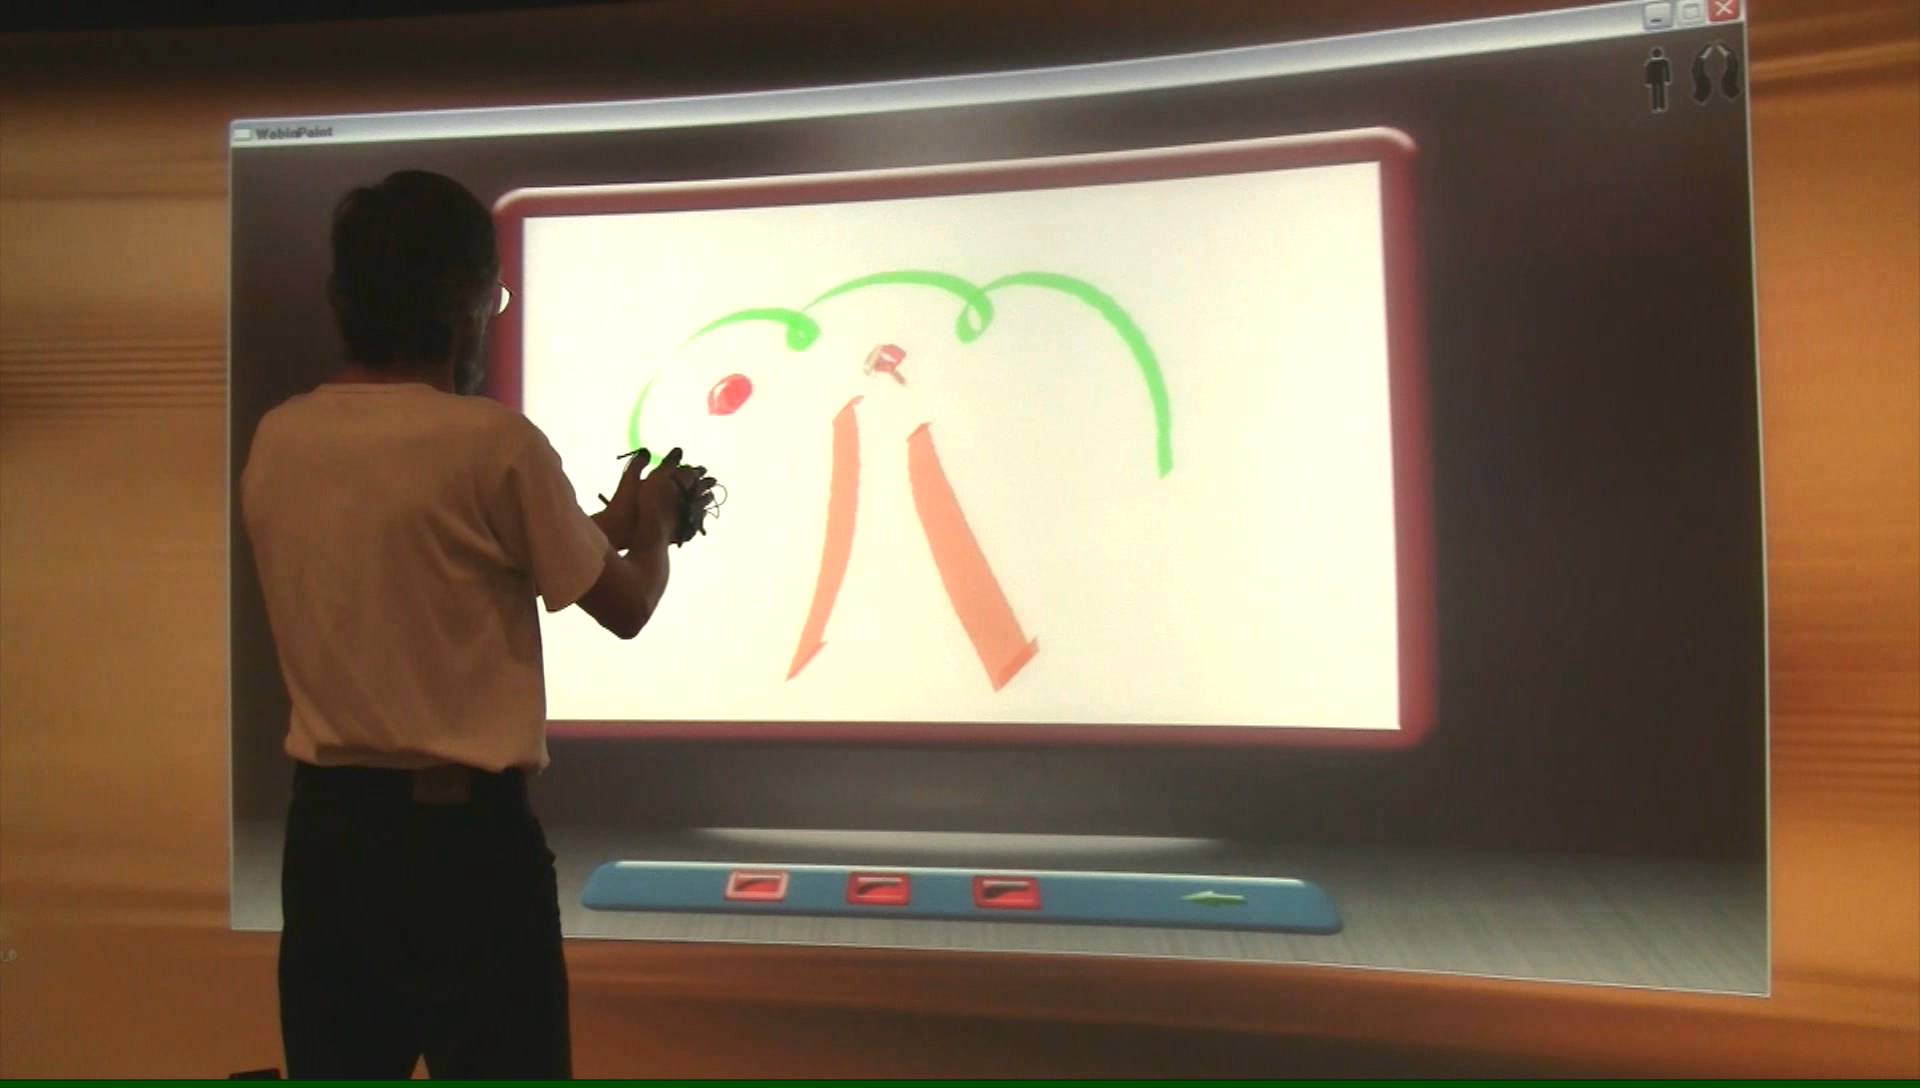
\includegraphics[scale=0.08]{images/WabinPaint.png}
	\end{center}
	\begin{itemize}
		\item application de dessin
		\item outils de dessin
		\item périphériques de tracking
	\end{itemize}
\end{frame}

\begin{frame}{Objectif}
	\begin{itemize}
		\item possibilité d'utiliser Kinect
		\item filtrer/lisser le signal obtenu par la Kinect		
	\end{itemize}
\end{frame}


\section{Analyse de l'existant}

\begin{frame}{Choix techniques}
	\begin{itemize}
		\item Clutter
			\begin{itemize}
				\item gére uniquement la souris
				\item tracker virtuel dans Wabinpaint emulant la souris
		\end{itemize}
		\item OpenNI
			\begin{itemize}
				\item utiliser serveur
				\item integrer client
		\end{itemize}
	\end{itemize}
\end{frame}

\begin{frame}{Mise en oeuvre}
	\begin{center}
		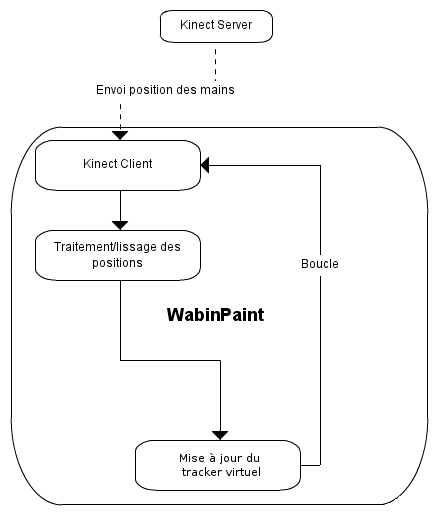
\includegraphics[scale=0.4]{images/plan.png}
	\end{center}
\end{frame}
\section{Kinect}

\subsection{Serveur}

\subsection{Client}



\section{Filtre}

\begin{frame}{Analyse}
	\begin{center}
		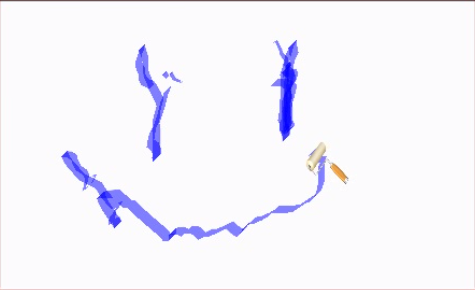
\includegraphics[scale=0.3]{images/bruit.png}
	\end{center}
	\begin{itemize}    
		\item tremblement du curseur
		\item filtre passe-bas
		\item latence possible -> algorithme de prediction
	\end{itemize}
\end{frame}

\begin{frame}{One Euro Filter}
	\begin{itemize}
		\item filtre passe-bas
		\item integration coté client
		\item latence
		\item reglage du filtre pour diminuer la latence
	\end{itemize}
\end{frame}

\section{Démo }


\section{Bilan}
\begin{frame}{Bilan et perspectives}
	\begin{itemize}
		\item Dead reckoning
		\item changement du mode dessin
	\end{itemize}
\end{frame}



\section{Conclusion}
\begin{frame}{Conclusion}
	\begin{itemize}
		\item Utilité de l'intégration continue
		\item Gain de temps pour la communauté
		\item Intérêt de la communauté
		\item Perspectives : 
		\begin{itemize}
			\item Ajout et amélioration des publieurs
			\item Ajout de règles, comme une contrainte de performance, benchmark
		\end{itemize}
	\end{itemize}
\end{frame}

\begin{frame}{Conclusion}
	\begin{columns}[T]
    		\begin{column}{.45\textwidth}
    			\begin{block}{Mémo}
    				\begin{itemize}
    					\item Gain de temps
    					\item Intérêt pour la communauté
    				\end{itemize}
    				\begin{itemize}
    					\item Contenu de CI
    					\begin{itemize}
    						\item Ligne de commande
    						\item Manageur
    						\item Validation
    						\item Publieur
    					\end{itemize}
    				\end{itemize}
    			\end{block}
    		\end{column}
    		\begin{column}{.5\textwidth}
   			\begin{block}{Fonctionnement de CI}
   				\begin{figure}
    					%\includegraphics[scale=0.4]{images/schema1.pdf}
   				\end{figure}
    			\end{block}
    		\end{column}
  \end{columns}
\end{frame}


\end{document}